\documentclass[aspectratio=169, 13pt]{beamer}
\usepackage[utf8]{inputenc}
\usepackage[english,russian]{babel}
\usepackage{graphicx}
\usepackage{sidecap}
\usepackage{mathtools}
\usepackage{appendixnumberbeamer}


\DeclarePairedDelimiter\bra{\langle}{\rvert}
\DeclarePairedDelimiter\ket{\lvert}{\rangle}
\DeclarePairedDelimiterX\braket[2]{\langle}{\rangle}{#1 \delimsize\vert #2}
\newcommand{\rbrkt}[1]{\left( #1 \right)}

\graphicspath{{../Pictures/}}
%beamer  theme's used to be here :)
\usetheme{mipt_beamer}
\usefonttheme[onlymath]{serif}

\title{Исследование сверхпроводящих потоковых кубитов}
\author{Федоров~Г.\quad Научный руководитель: Шульга К. (Рязанов В.В.)}
\date{\today}

\setlength{\jot}{15pt}
\setbeamertemplate{footline}[page number]
\renewcommand*{\inserttotalframenumber}{\insertpresentationendpage}

\AtBeginSection[]
{
  \begin{frame}[plain]
    \tableofcontents[currentsection]
    \addtocounter{page}{-1}
  \end{frame}
}



\begin{document}

{
\begin{frame}[plain]
  \titlepage
\end{frame}
}

\frame[plain]{\tableofcontents}

\section{Теоретические сведения}
\subsection{Квантовые биты}
\begin{frame}[c]\frametitle{\secname}\framesubtitle{\subsecname}
\begin{columns}[c]
\column{0.5\textwidth}
\centering
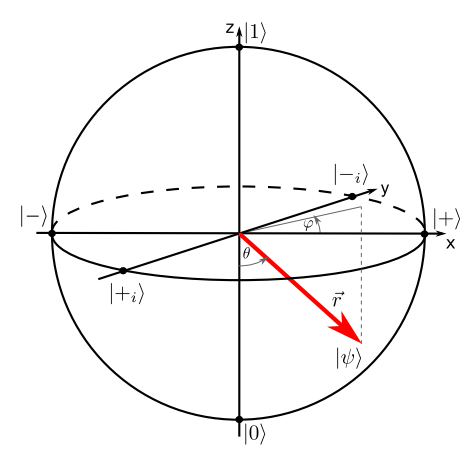
\includegraphics[width=0.85\textwidth]{bloch_sphere}

Сфера Блоха

\column{0.5\textwidth}
Состояние классического бита:
\begin{equation*}
0\ \text{или}\ 1
\end{equation*}
Состояние квантового бита:
\hspace{-2cm}
\begin{equation*}
\ket{\psi} = a\ket{0}+b\ket{1},\ a,b \in \mathbb{C}
\end{equation*}
\end{columns}
\end{frame}



\subsection{Теория изолированного Flux-кубита}
\begin{frame}[c]\frametitle{\secname}\framesubtitle{\subsecname}

\vspace{-1cm}
\only<1>{

\vspace{0.5cm}
Степени свободы: 
\begin{equation*}
\varphi_1,\ \varphi_2,\ \varphi_3 = 2\pi\frac{\Phi}{\Phi_0} - \varphi_1 - \varphi_2 \ (\text{квантование }\Phi,\ \varphi_3\ \text{зависима от первых двух})
\end{equation*}
}

\only<1>{
\begin{columns}[c]
\column{0.5\textwidth}
Энергия одного перехода:
\hspace{-1cm}
\begin{align*}
E_i = E_J(1-\cos\varphi_i) + \frac{\hbar^2}{4E_C} \dot \varphi_i^2, \\ 
E_J = \frac{\hbar}{2e}I_c,\ E_C = \frac{(2e)^2}{2C}
\end{align*}

\column{0.5\textwidth}
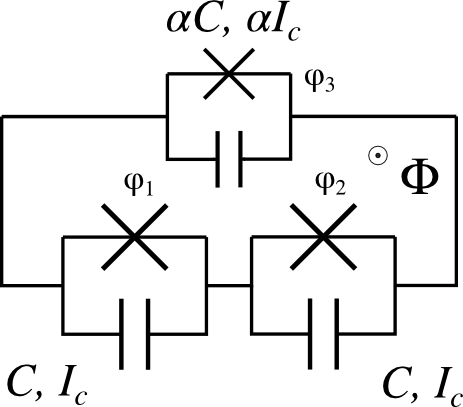
\includegraphics[width = 0.75\textwidth]{qubit}

\end{columns}
}
\only<2>{

\begin{columns}[t]
\column{0.5\textwidth}

\vspace{1cm}
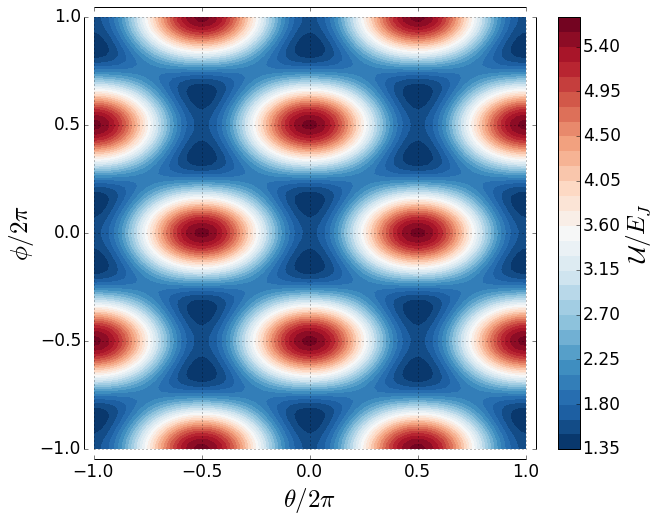
\includegraphics[width=\textwidth]{qubit_potential}

\column{0.5\textwidth}

\vspace{1cm}
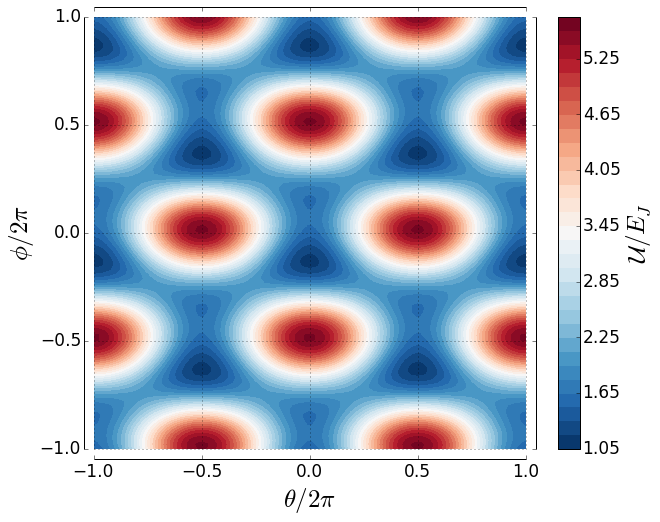
\includegraphics[width=\textwidth]{qubit_potential2}

\end{columns}

\begin{gather*}
 U = E_J\bigg[2+\alpha - 2\cos(\phi)\cos(\theta) 
-\left. \alpha\cos\left(2\pi\frac{\Phi}{\Phi_0} -2\phi \right)\right], \phi = \frac{\varphi_1+\varphi_2}{2}, \theta=\frac{\varphi_1 - \varphi_2}{2}
\end{gather*}
}

\end{frame}

\subsection{Энергетический спектр Flux-кубита}
\begin{frame}[c]\frametitle{\secname}\framesubtitle{\subsecname}
\only<1>{
\begin{columns}[c]

\column{\textwidth}

\vspace{0cm}
\centering
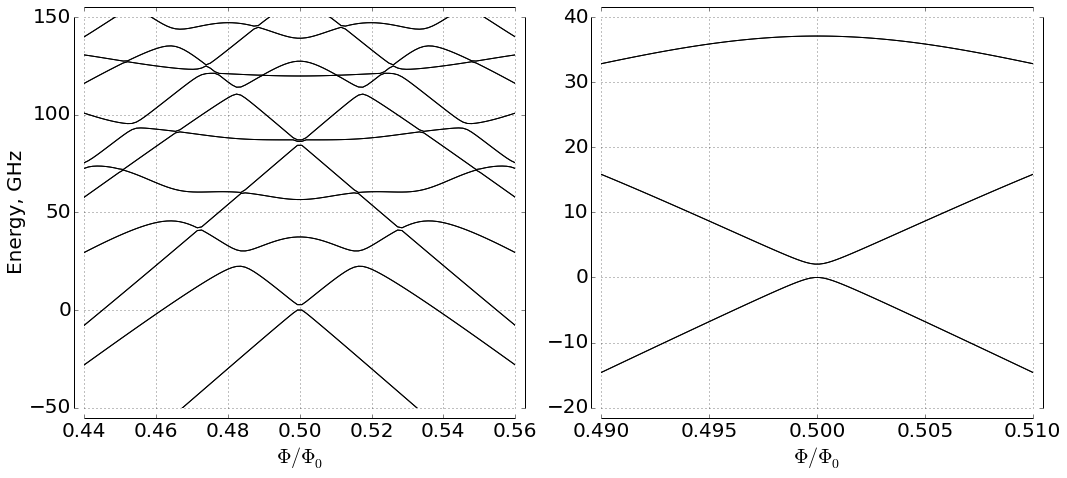
\includegraphics[width=0.7\textwidth]{qubit_levels}
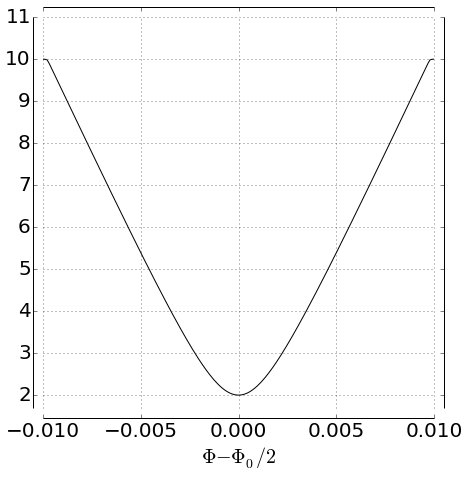
\includegraphics[width=0.307\textwidth]{spectrum_hyp}
\begin{gather*}
\hat{\mathcal{H}} = \frac{\varepsilon}{2}\,\hat\sigma_z + \frac{\delta}{2}\,\hat\sigma_x,\ 
E_1 - E_0 = \sqrt{\varepsilon^2+\delta^2} \text{ -- гипербола по }\delta
 \\ \small{ \ket{0}_{\Phi_0/2}=\rbrkt{\begin{matrix}
1 & 0\end{matrix}}^T,\ \ket{1}_{\Phi_0/2}=\rbrkt{\begin{matrix}
0 & 1\end{matrix}}^T,\ \delta \propto \Phi-\Phi_0/2}
\end{gather*}
\end{columns}
}
\end{frame}


\subsection{Кубит, связанный с резонатором}
\begin{frame}[c]\frametitle{\secname}\framesubtitle{\subsecname}
\begin{columns}[c]

\column{0.5\textwidth}
\centering
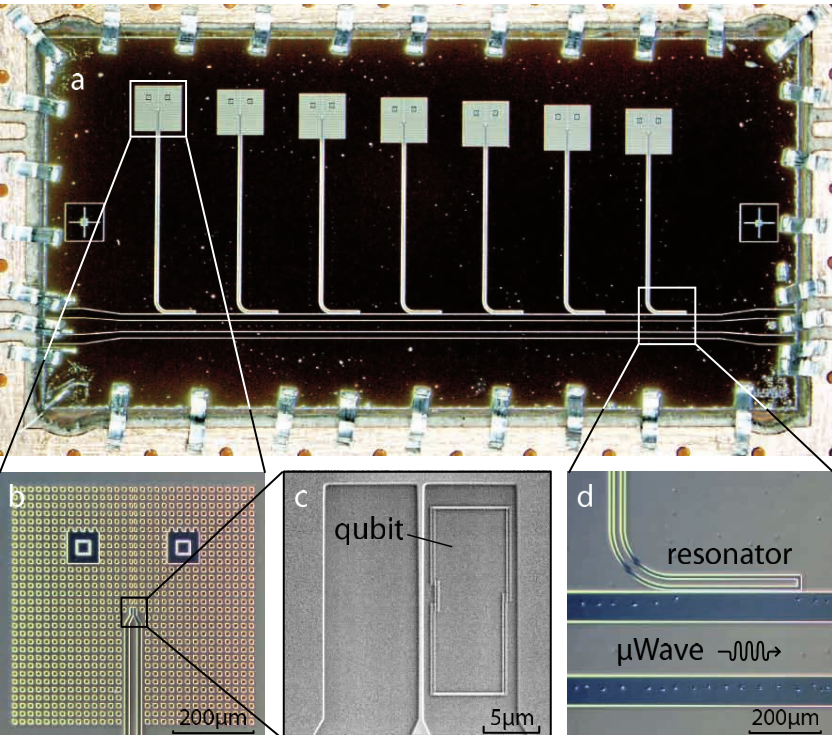
\includegraphics[width=\textwidth]{marcus_chip}
\column{0.5\textwidth}
Ситуация при $\Phi = \Phi_0/2$:
\begin{gather*}
\hat{\mathcal{H}} = \hat{\mathcal{H}}_{q}+\hat{\mathcal{H}}_{r}+\hat{\mathcal{H}}_{i},\\
\hat{\mathcal{H}}_{q} = \frac{\varepsilon}{2} \hat{\sigma_z} = \frac{\hbar\omega_q}{2}\hat{\sigma_z},\\
\hat{\mathcal{H}}_{r} = \hbar\omega_r \hat a^+ \hat{a}, \\
\hat{\mathcal{H}}_{i} = 
\begin{cases} 
g(\hat a^+ + \hat{a})\hat{\sigma}_x = g(\hat a^+ + \hat{a})(\hat\sigma^++\hat\sigma^-) \\ 
g(\hat a \hat\sigma^- + \hat{a}\hat\sigma^+)\ \text{, в приближении}
\end{cases}
\end{gather*}
\hspace{1cm} -- модель Джейнса-Каммингса

\end{columns}
\end{frame}

\section{Экспериментальные методы}
\subsection{Установка}
\frame{\frametitle{\secname}\framesubtitle{\subsecname}
\begin{columns}[c]
\column{\textwidth}
Взаимодействие с образцом внутри криостата:
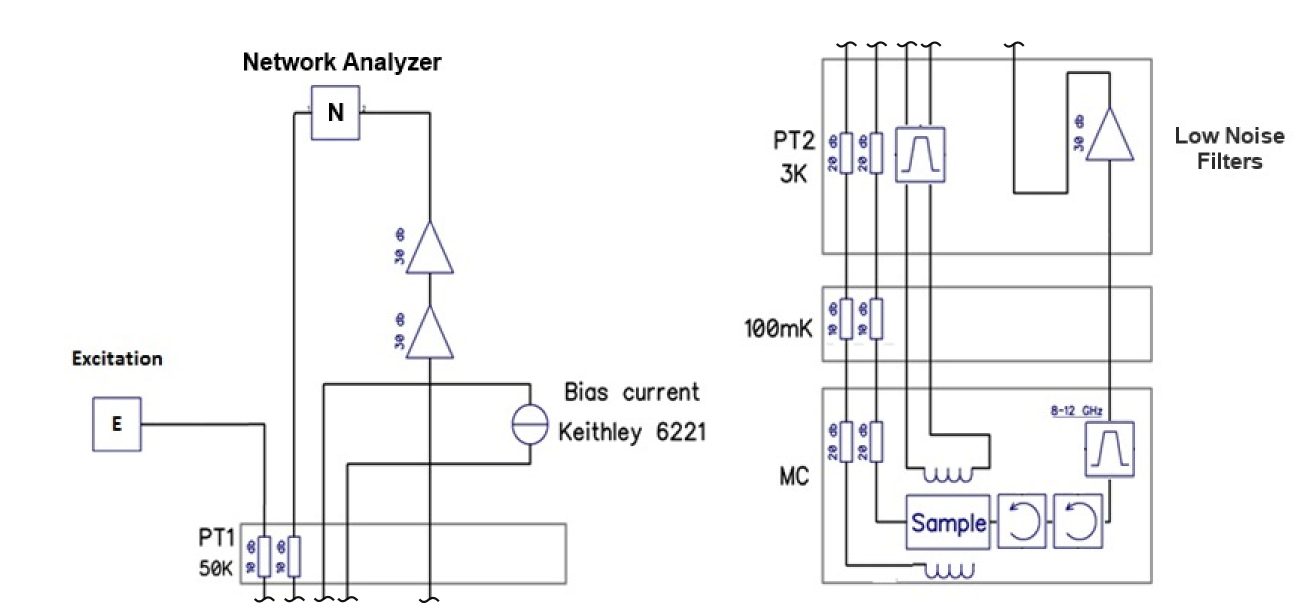
\includegraphics[width=\textwidth]{crio_scheme}
\end{columns}
}
\subsection{Техника измерений}
\frame{\frametitle{\secname}\framesubtitle{\subsecname}
\begin{columns}[c]
\column{0.5\textwidth}

\vspace{-1cm}
В эксперименте фактически наблюдаются сдвиги или расщепления частот поглощения:

\vspace{0.5cm}
\centering
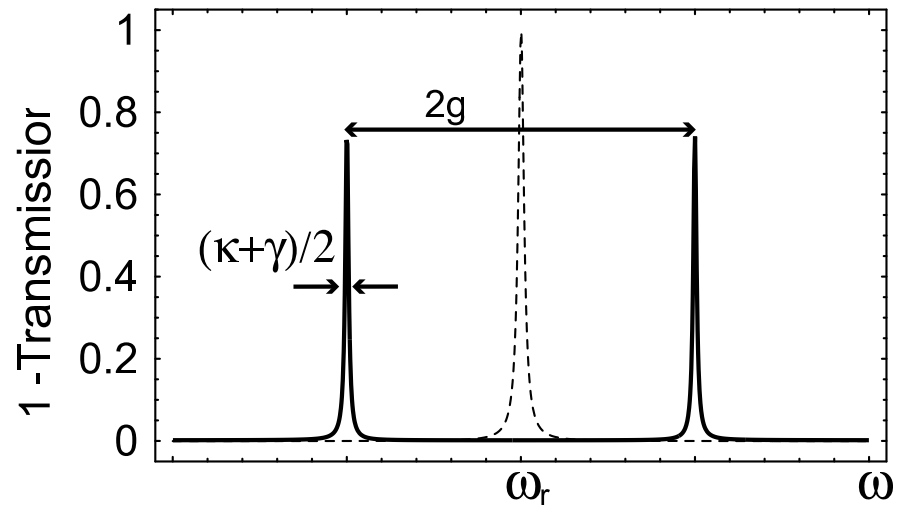
\includegraphics[width=\textwidth]{frequency_shift}
\column{0.5\textwidth}
\centering
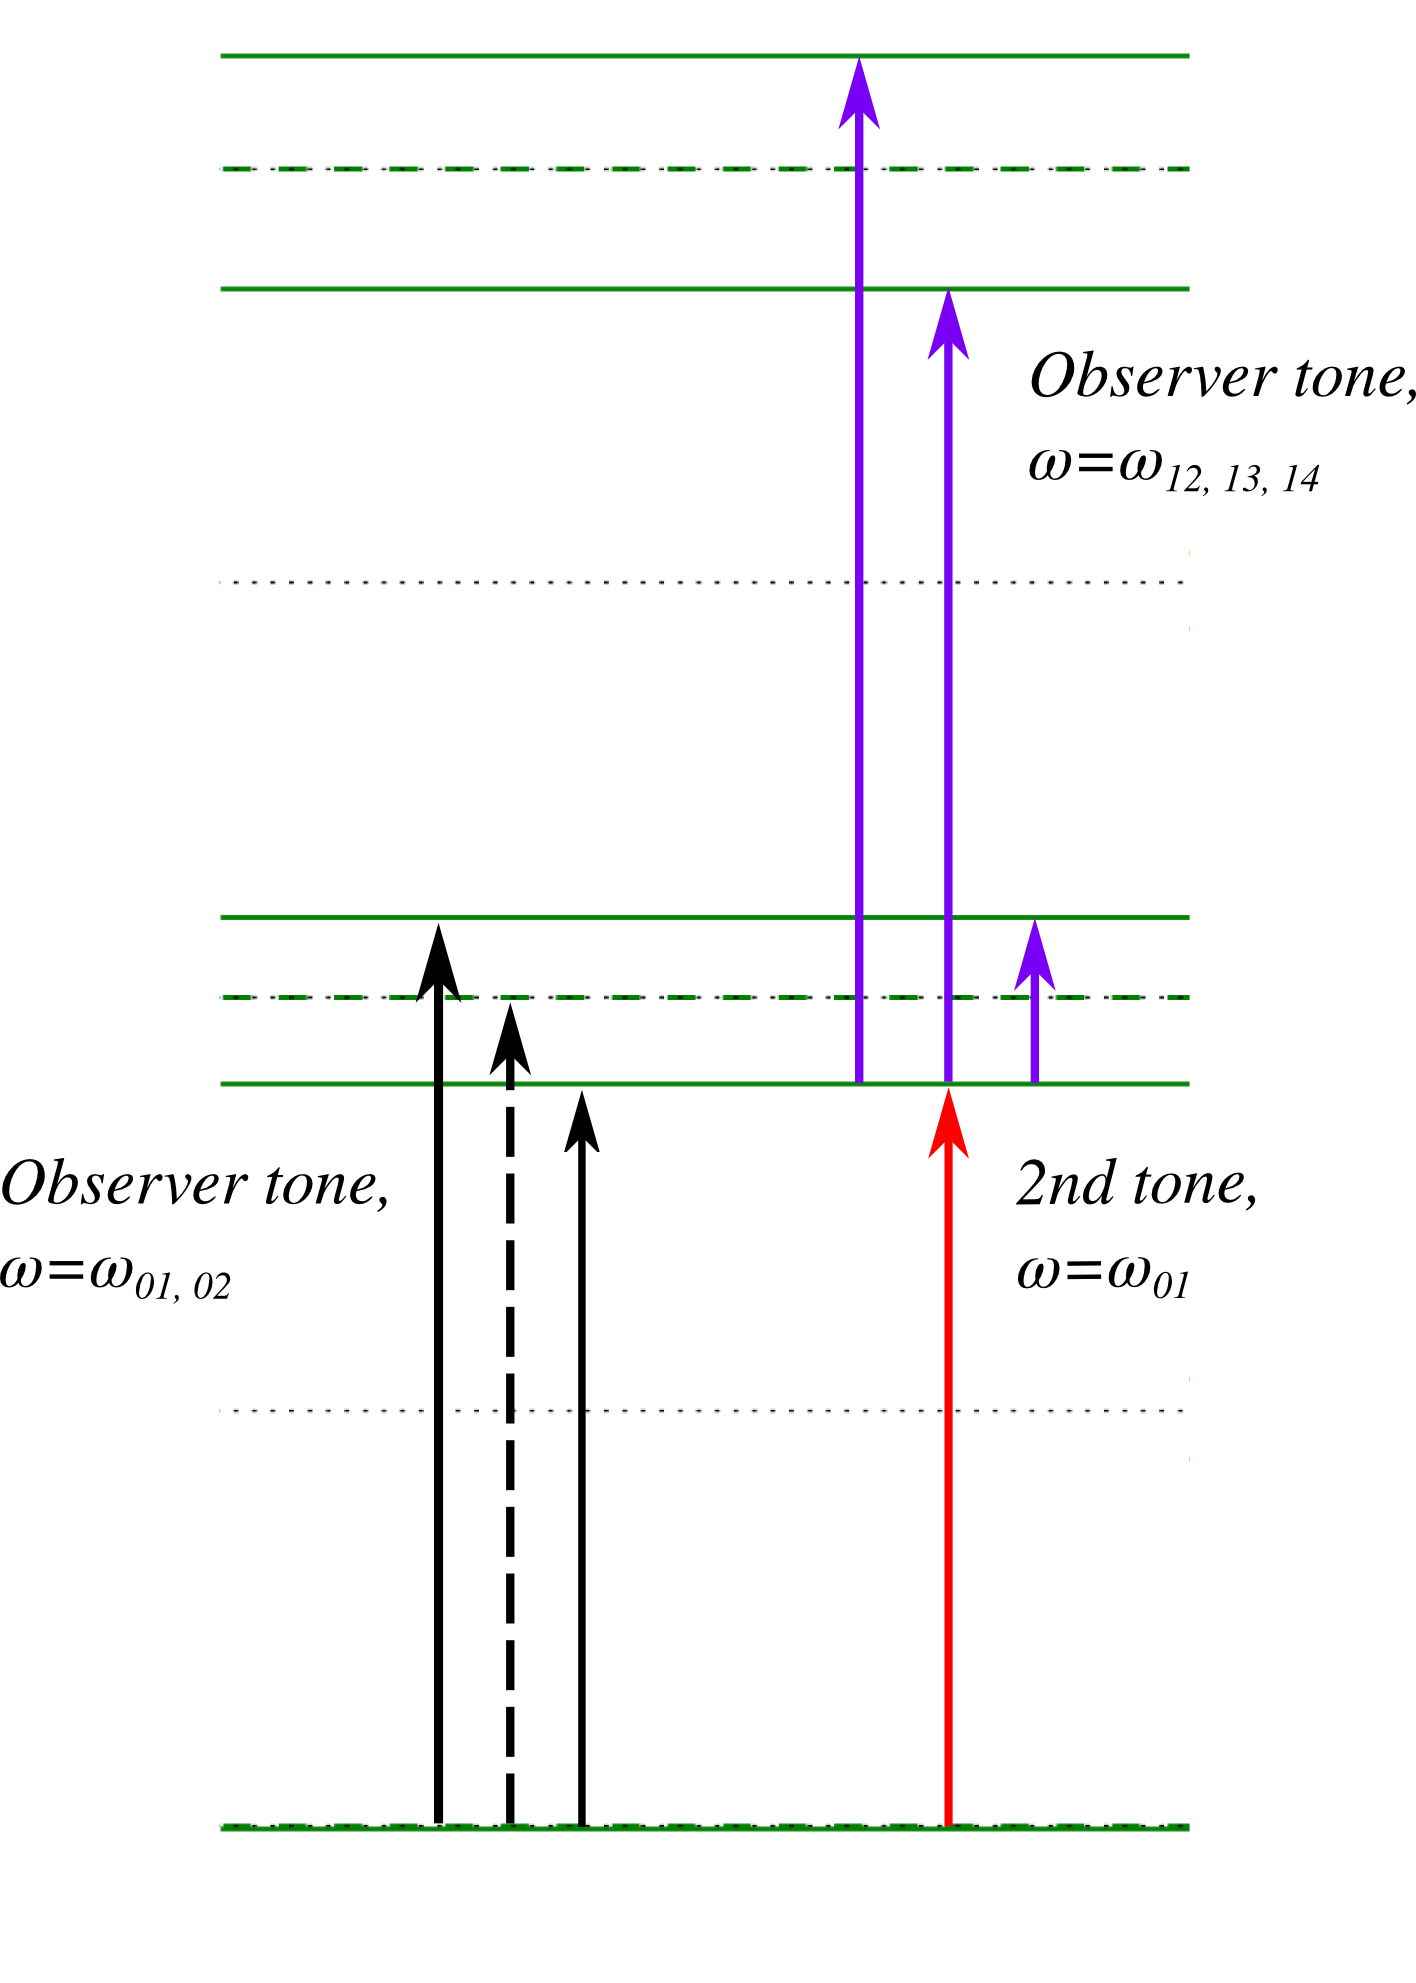
\includegraphics[height=0.85\textheight]{2tone}

\end{columns}
}
\section{Результаты}
\subsection{Спектры}
\frame{\frametitle{\secname}\framesubtitle{\subsecname}
\vspace{0.5cm}
\begin{columns}[c]

\hspace*{-0.5cm}
\column{0.5\textwidth}
\centering
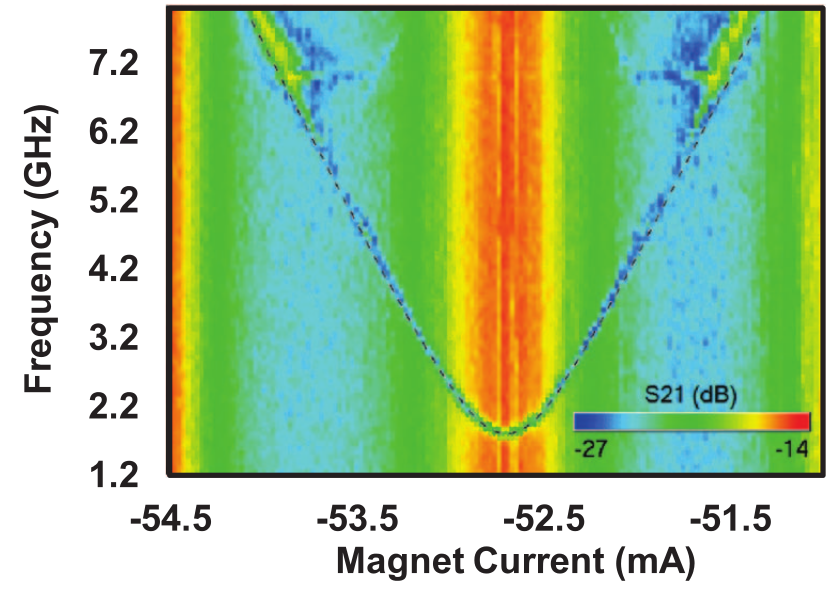
\includegraphics[width=\textwidth]{sin}

\column{0.5\textwidth}
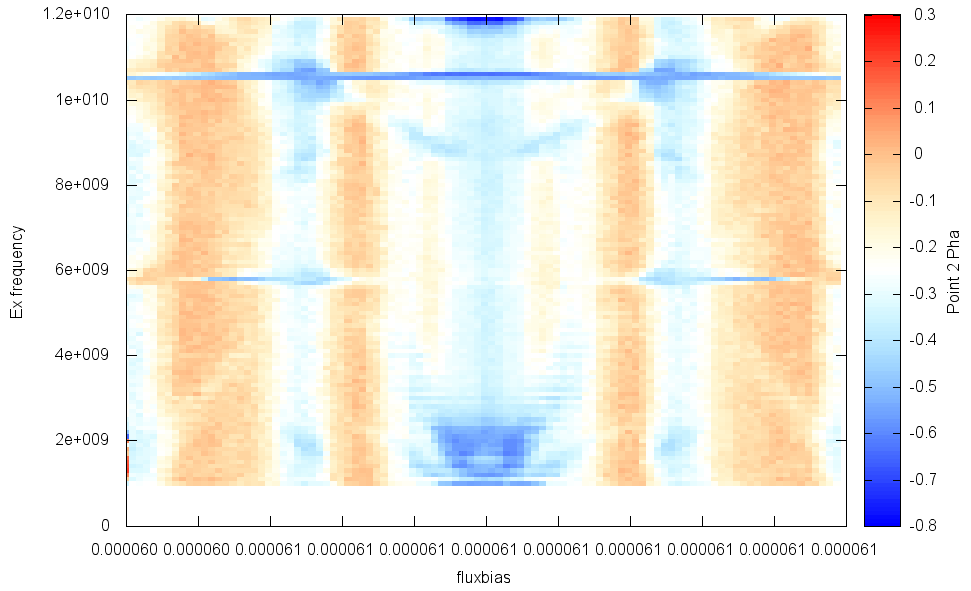
\includegraphics[width=\textwidth]{spectrum}

\end{columns}

\vspace{0.5cm}
Гиперболическая зависимость от $\delta\propto \Phi - \Phi_0/2$:
\centering
\begin{equation*}
\hbar \omega_{01} = \sqrt{\varepsilon^2+\delta^2}
\end{equation*}
}
\subsection{Наблюдение квазипересечения уровней}
\frame{\frametitle{\secname}\framesubtitle{\subsecname}
\begin{columns}[c]
\column{\textwidth}
\centering
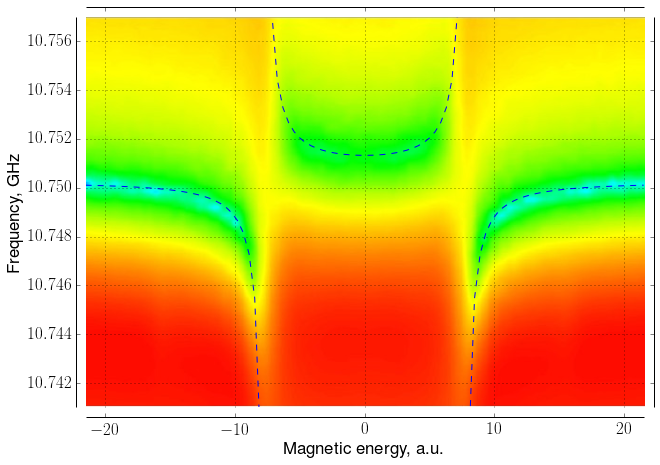
\includegraphics[width=0.75\textwidth]{qintersect}
\end{columns}
}
\subsection{Нелинейные эффекты}
\frame{\frametitle{\secname}\framesubtitle{\subsecname} 
\begin{columns}[c]
\column{\textwidth}
\centering
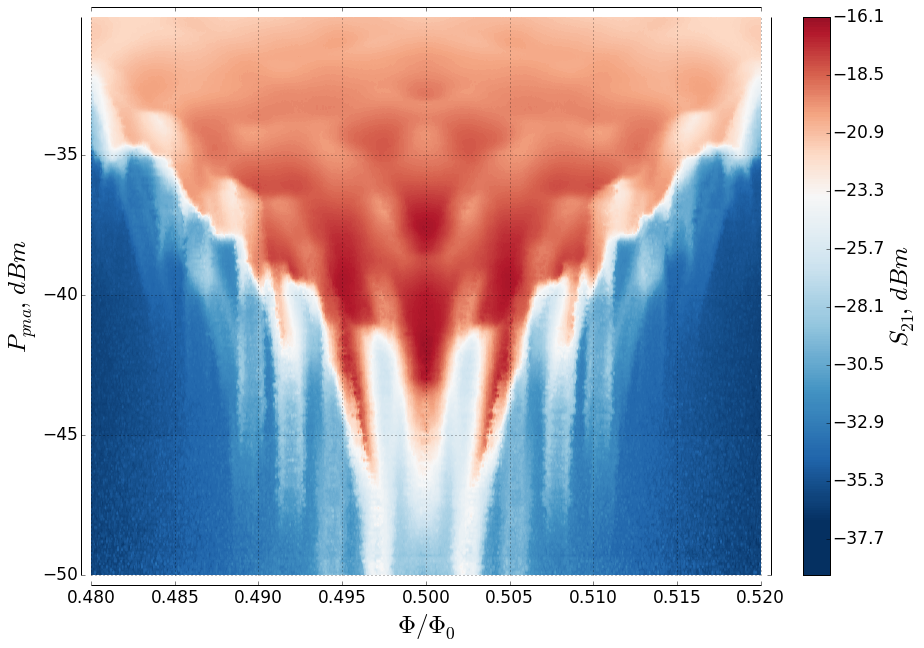
\includegraphics[width=0.75\textwidth]{LZI}
\end{columns}
}


\appendix

\section*{Вспомогательные материалы}
\subsection*{Сверхпроводимость и эффект Джозефсона}
\begin{frame}[noframenumbering, c, label=1st]\frametitle{\secname}\framesubtitle{\subsecname}
\addvspace{-2cm}

\begin{columns}[c]
\column{0.5\textwidth}

\vspace{1.2cm}
\only<1>{Теория Г.-Л. и уравнения Джозефсона:}
\only<2>{Квантование магнитного потока:}
\begin{gather*}
\Psi(\mathbf{r}) = \sqrt{\frac{n_s}{2}}e^{i\theta(\mathbf{r})}\\
\only<1>{
I_s = I_c\sin\varphi,\ \hbar\frac{\partial\varphi}{\partial t} = 2eV \\
E = E_J(1-\cos\varphi) + \frac{\hbar^2}{4E_C} \dot \varphi^2, \\ 
E_J = \frac{\hbar}{2e}I_c,\ E_C = \frac{(2e)^2}{2C}
}
\only<2>{
\mathbf{j}_s = \frac{1}{\Lambda}\left(\frac{\Phi_0}{2\pi}\nabla\theta(\mathbf{r})-\mathbf{A}\right)\\
\sum_i \varphi_n = 2\pi\left(\frac{\Phi}{\Phi_0} - k\right),\ k\in \mathcal{Z},\\
\Phi_0 = \frac{h}{2e}
}
\end{gather*}
\column{0.5\textwidth}

\vspace{1cm}
\only<1>{
\centering
Разность фаз на берегах контакта: \\
$\Delta \theta = \varphi$

\vspace{0.2cm}
\hspace{-.2cm}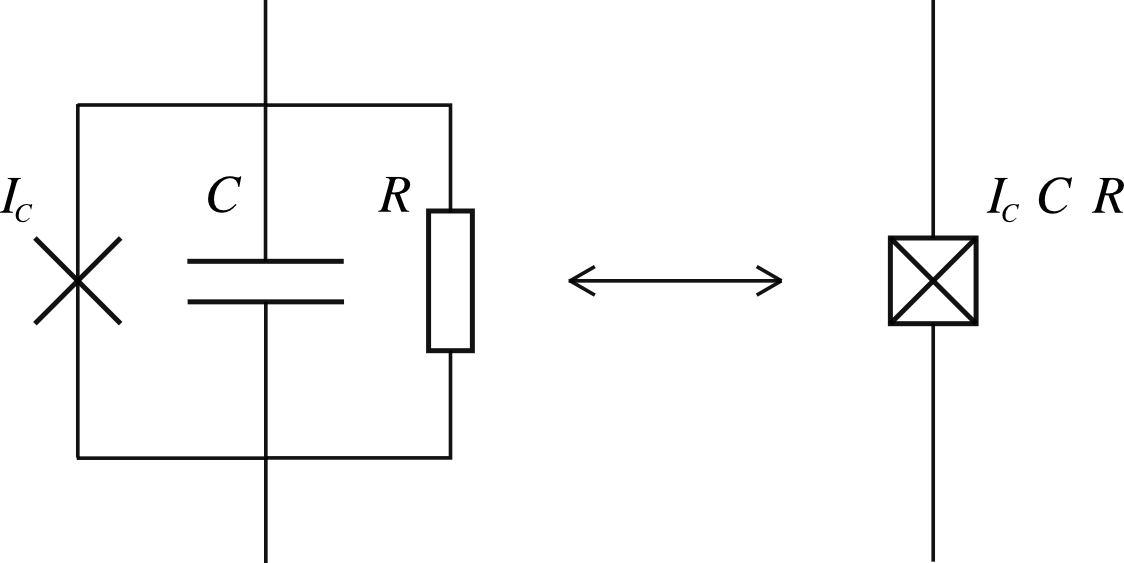
\includegraphics[width=1.05\textwidth]{RCSJ} 

RSCJ-модель
}
\only<2>{\vspace{1cm}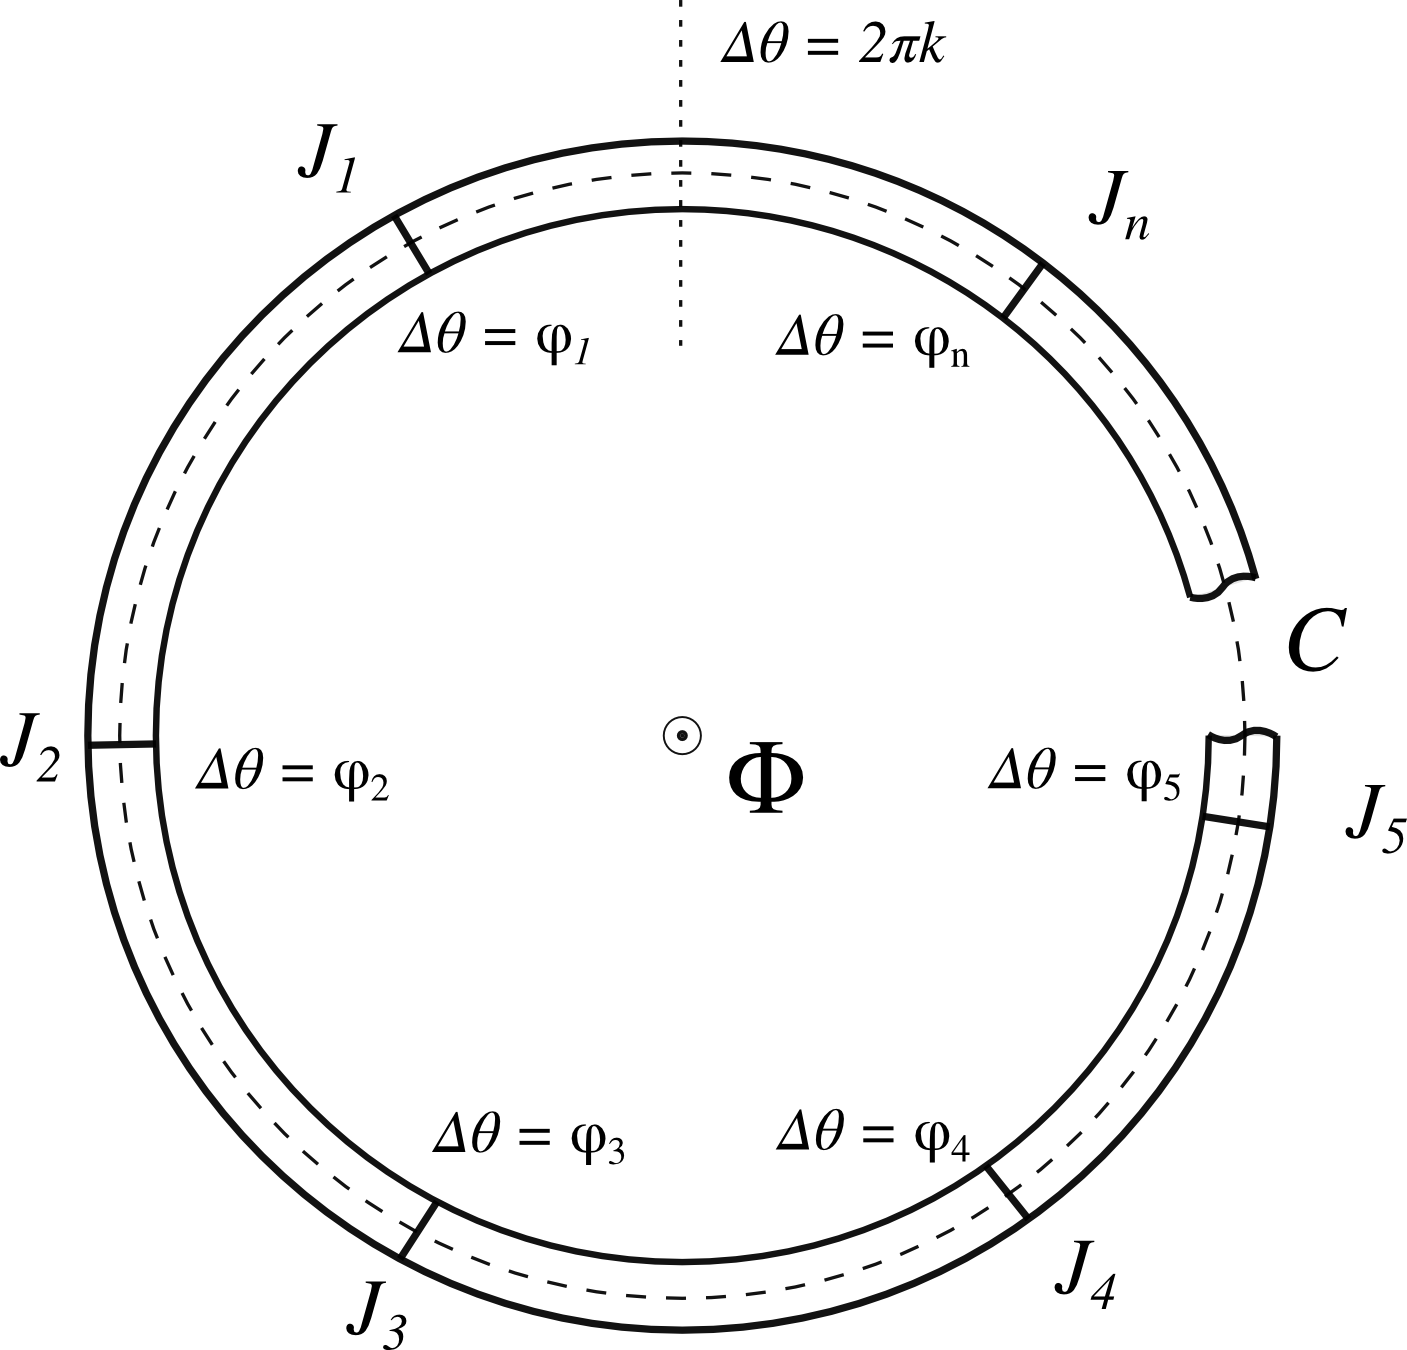
\includegraphics[width=0.9\textwidth]{ring}}
\end{columns}
\end{frame}

\subsection*{Энергетический спектр модели Д.-К.}
\begin{frame}[c, noframenumbering]\frametitle{\secname}\framesubtitle{\subsecname}
\begin{columns}
\only<1>{
\column{\textwidth}
\centering
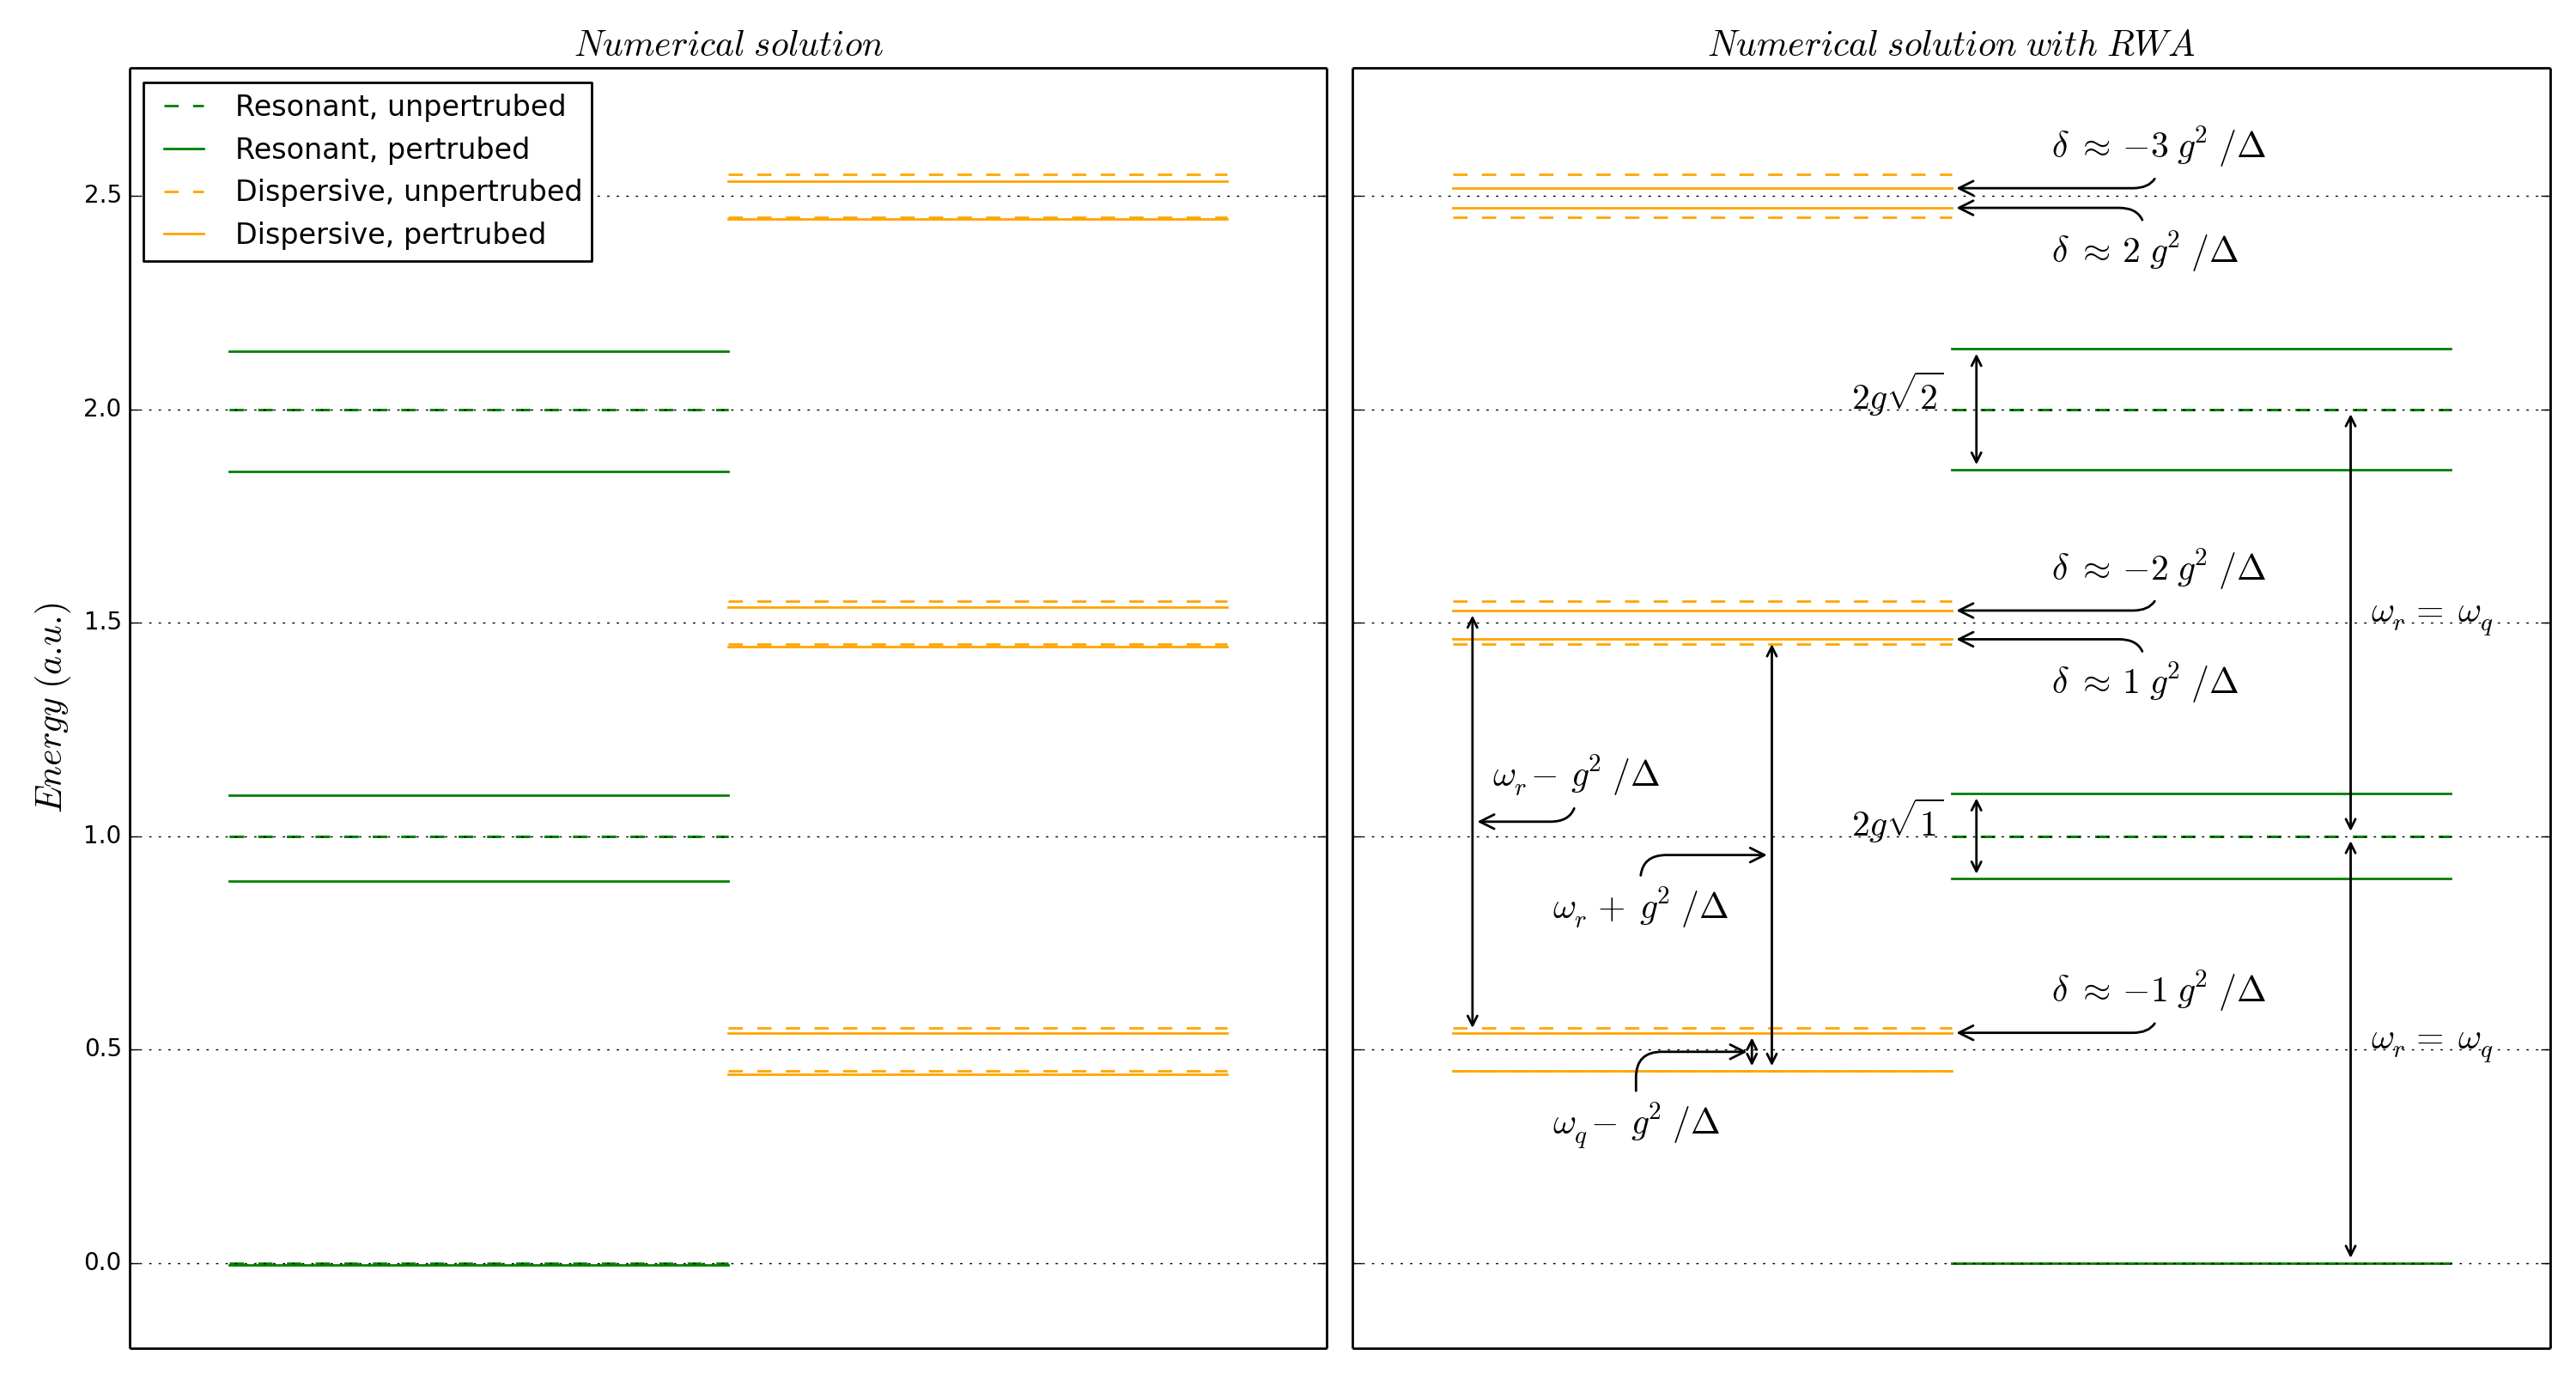
\includegraphics[width=1\textwidth]{JCM_levels}
}
\only<2>{
\column{0.5\textwidth}

\hspace{-1cm}
\centering
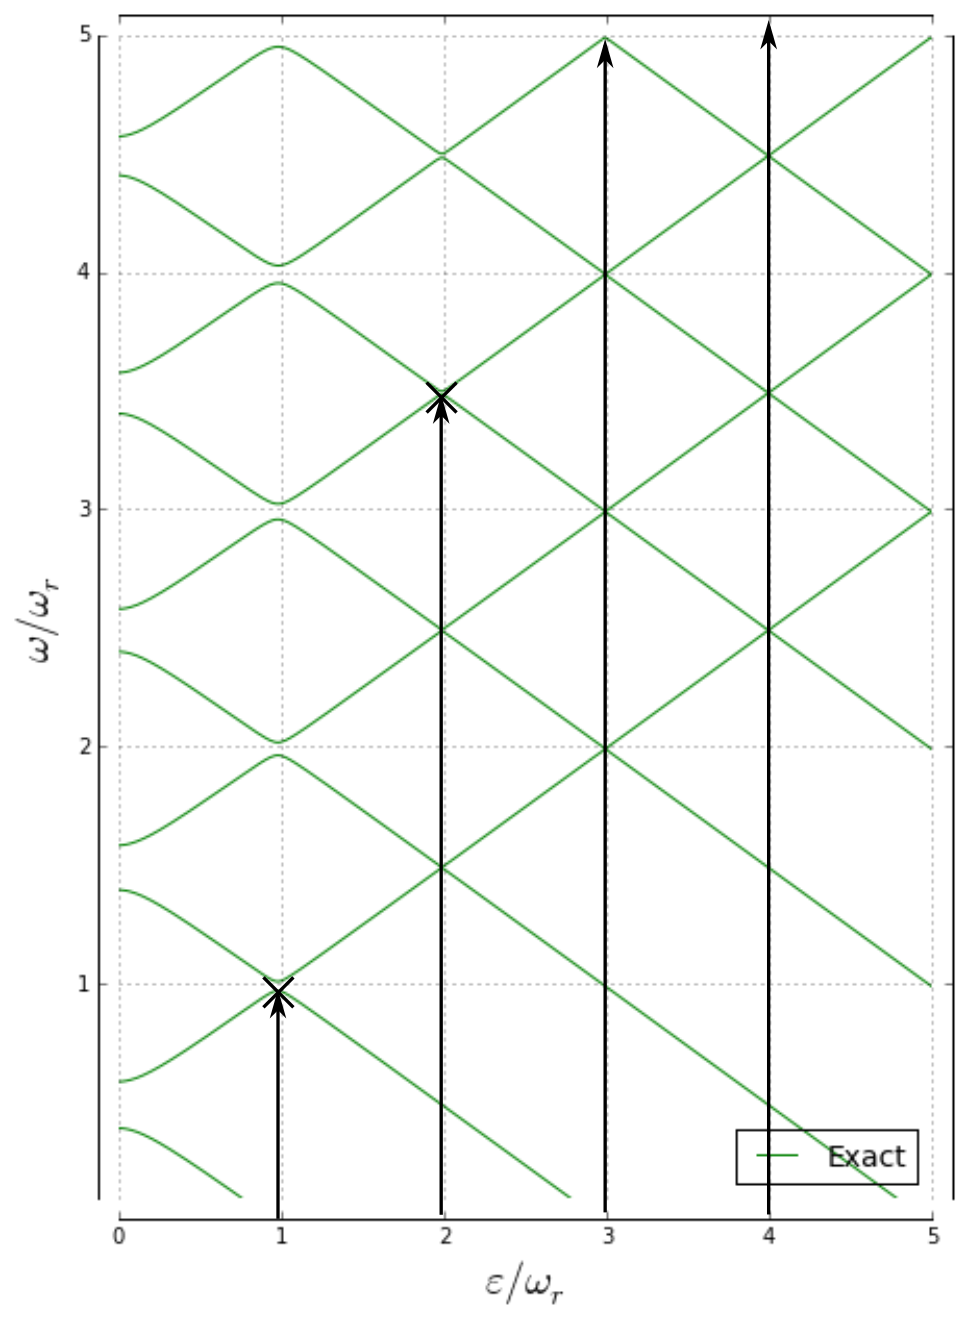
\includegraphics[height=0.8\textheight]{JCM_MF}
\column{0.5\textwidth}

\centering
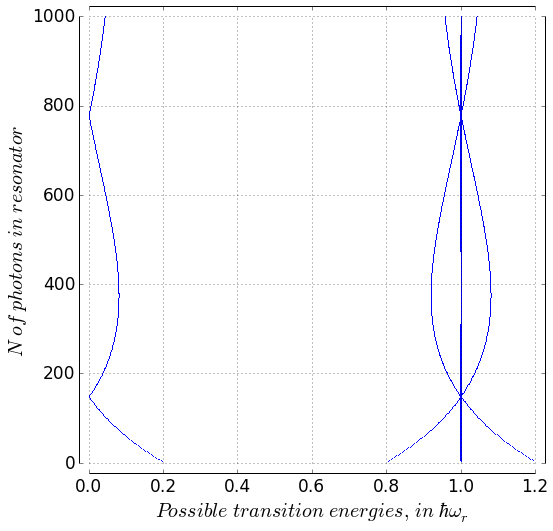
\includegraphics[height=0.8\textheight]{JCM_transitions}
}
\end{columns}
\end{frame}


\end{document}